\documentclass[conference]{IEEEtran}
\IEEEoverridecommandlockouts

\usepackage{cite}
\usepackage{amsmath,amssymb,amsfonts}
\usepackage{graphicx}
\usepackage{textcomp}
\usepackage{xcolor}
\usepackage{hyperref}

% Robust PDF bookmarks: keep acronym commands out of bookmark strings.
\pdfstringdefDisableCommands{%
  \def\ac#1{#1}%
  \def\acs#1{#1}%
  \def\acf#1{#1}%
  \def\acp#1{#1}%
  \def\Acp#1{#1}%
}
\usepackage{booktabs}
\usepackage{multirow}
\usepackage{microtype}
\usepackage[nohyperlinks]{acronym}
% Acronym definitions. Use \newacro in the preamble so acronyms are available on the first LaTeX pass.
% This avoids the acronym package's undefined-acronym fallback, which appears as bold text followed by an exclamation mark.
\renewcommand*{\aclabelfont}[1]{#1}
\newacro{AI}[AI]{artificial intelligence}
\newacro{HPC}[HPC]{high-performance computing}
\newacro{MLIP}[MLIP]{machine-learned interatomic potential}
\newacro{DFT}[DFT]{density functional theory}
\newacro{AL}[AL]{active learning}
\newacro{LLM}[LLM]{large language model}
\newacro{QE}[QE]{Quantum ESPRESSO}
\newacro{VASP}[VASP]{Vienna Ab initio Simulation Package}
\newacro{DOE}[DOE]{Department of Energy}
\newacro{NERSC}[NERSC]{National Energy Research Scientific Computing Center}
\newacro{OLCF}[OLCF]{Oak Ridge Leadership Computing Facility}
\newacro{ALCF}[ALCF]{Argonne Leadership Computing Facility}
\newacro{GNN}[GNN]{graph neural network}
\newacro{MLP}[MLP]{multilayer perceptron}
\newacro{MAE}[MAE]{mean absolute error}
\newacro{MC}[MC]{Monte Carlo}
\newacro{MD}[MD]{molecular dynamics}
\newacro{ASE}[ASE]{Atomic Simulation Environment}
\newacro{FIRE}[FIRE]{Fast Inertial Relaxation Engine}
\newacro{BFGS}[BFGS]{Broyden--Fletcher--Goldfarb--Shanno}
\newacro{SCF}[SCF]{self-consistent field}
\newacro{RMS}[RMS]{root mean square}
\newacro{BCC}[BCC]{body-centered cubic}
\newacro{HEA}[HEA]{high-entropy alloy}
\newacro{GGA}[GGA]{generalized-gradient approximation}
\newacro{MOF}[MOF]{metal--organic framework}
\newacro{GPU}[GPU]{graphics processing unit}
\newacro{CUDA}[CUDA]{Compute Unified Device Architecture}
\newacro{MPI}[MPI]{Message Passing Interface}
\newacro{PVC}[PVC]{Ponte Vecchio}
\newacro{GCD}[GCD]{graphics compute die}
\newacro{NVT}[NVT]{constant-particle-number, constant-volume, constant-temperature}
\newacro{REPL}[REPL]{read--eval--print loop}
\newacro{JSON}[JSON]{JavaScript Object Notation}
\newacro{JSONL}[JSONL]{JavaScript Object Notation Lines}
\newacro{HTTP}[HTTP]{Hypertext Transfer Protocol}
\newacro{NLP}[NLP]{natural language processing}
\newacro{FFTW}[FFTW]{Fastest Fourier Transform in the West}
\newacro{ELPA}[ELPA]{Eigenvalue SoLvers for Petaflop-Applications}
\newacro{GTL}[GTL]{GPU transport layer}
\newacro{XPU}[XPU]{Intel accelerated processing unit}
\newacro{DFTB}[DFTB]{density-functional tight binding}
\newacro{GFM}[GFM]{graph foundation model}
\newacro{MTL}[MTL]{multi-task learning}
\newacro{MPNN}[MPNN]{message-passing neural network}
\newacro{ADIOS2}[ADIOS2]{Adaptable Input/Output System 2}
\newacro{DDStore}[DDStore]{Distributed Data Store}
\newacro{NVMe}[NVMe]{non-volatile memory express}
\newacro{FP64}[FP64]{64-bit floating point}
\newacro{FP32}[FP32]{32-bit floating point}
\newacro{BF16}[BF16]{bfloat16}
\usepackage{tikz}
\usetikzlibrary{shapes.geometric, arrows.meta, positioning, fit, backgrounds}

\def\BibTeX{{\rm B\kern-.05em{\sc i\kern-.025em b}\kern-.08em
    T\kern-.1667em\lower.7ex\hbox{E}\kern-.125emX}}

\begin{document}

% =============================================================================
\title{A Scalable Agentic Artificial Intelligence Scientific Workflow for
Atomistic Materials Characterization}

\author{
\IEEEauthorblockN{Massimiliano Lupo Pasini\textsuperscript{1} (corresponding author), Zekun Chen\textsuperscript{2}, Anubhav Jain\textsuperscript{2}}
\IEEEauthorblockA{\textsuperscript{1}Computational Sciences and Engineering Division, Oak Ridge National Laboratory}
\IEEEauthorblockA{\textsuperscript{2}Energy Storage \& Distributed Resources Lawrence Berkeley National Laboratory}\IEEEauthorblockA{lupopasinim@ornl.gov, zchen11@lbl.gov ajain@lbl.gov}
}

\maketitle

% =============================================================================
\begin{abstract}
We present \textsc{matsim-agents}, a fault-tolerant, backend-portable agentic
\ac{AI} workflow that translates natural-language scientific objectives into
typed, auditable atomistic-simulation plans on leadership-class \ac{HPC}. A
checkpointed \acs{LLM}-driven orchestration layer couples fast \ac{MLIP}
exploration, selective first-principles (\acs{DFT}) labeling, and model
adaptation, treating both the \ac{MLIP} and the \acs{DFT} engine as
configuration-selected backends (HydraGNN, UMA, and MACE-MP potentials; \ac{QE}
and \ac{VASP}). The \acs{LLM} plans and interprets evidence, while explicit
scientific-computation stages produce every physical quantity and rule-based gates
decide when to escalate to \acs{DFT}. Across five unattended end-to-end campaigns
on \ac{NERSC} Perlmutter the loop runs without manual intervention and resumes across batch
allocations; single-point \acs{DFT} labeling accounts for $88$--$97\%$ of
iteration wall time while all non-\acs{DFT} stages combined account for
$3$--$12\%$, and the dominant \acs{DFT} stage scales from one to eight nodes at
$74$--$79\%$ parallel efficiency. We further show that measured surrogate accuracy
can drive an auditable decision to continue \acs{MLIP} screening or escalate
to first-principles calculations, and we characterize backend- and
material-dependent fine-tuning and warm-start behavior across positive, neutral,
and negative outcomes.
\end{abstract}

\begin{IEEEkeywords}
agentic artificial intelligence, materials discovery, machine learning force field, HydraGNN,
UMA, MACE, fairchem-core, universal MLIP,
active learning, Quantum ESPRESSO, VASP,
warm-start, high-performance computing, scientific workflow
\end{IEEEkeywords}

{\footnotesize{This manuscript has been authored in part by UT-Battelle, LLC, under contract DE-AC05-00OR22725 with the US Department of Energy (DOE). The US government retains and the publisher, by accepting the article for publication, acknowledges that the US government retains a nonexclusive, paid-up, irrevocable, worldwide license to publish or reproduce the published form of this manuscript, or allow others to do so, for US government purposes. DOE will provide public access to these results of federally sponsored research in accordance with the DOE Public Access Plan (\url{http://energy.gov/downloads/doe-public-access-plan}).}}

% =============================================================================
\section{Introduction}
\label{sec:intro}

Accelerating the discovery of novel functional materials remains one of the
grand challenges at the intersection of computational science and
\acs{HPC}. First-principles electronic-structure methods such
as \acs{DFT} provide accurate energies and forces but scale as $\mathcal{O}(N^3)$ in
the number of electrons and are therefore prohibitively expensive for
high-throughput exploration of large chemical spaces. \Acp{MLIP}~\cite{behler2007,bartok2010,batzner2022} offer
near-\acs{DFT} accuracy at a fraction of the cost, but their reliability degrades
silently outside the training distribution, making undetected extrapolation a
practical risk in autonomous workflows.

Agentic \acs{AI} provides a mechanism for coordinating these tasks through
planning, tool invocation, conditional branching, and repeated evaluation. By
embedding an \ac{MLIP} within a workflow that can escalate selected
configurations to \acs{DFT}, the system can use the surrogate for broad
exploration while reserving first-principles calculations for configurations
that require higher-fidelity evaluation.

Existing \acs{AL} workflows for \acp{MLIP}~\cite{smith2018,vandermause2020,
podryabinkin2017} already automate candidate generation, \acs{DFT} labeling, and
retraining, and recent agentic tools add \acs{LLM}-driven planning on top.
Several practical challenges remain for deployment on leadership-class
\acs{HPC}. Many workflows are tied to a particular surrogate or
first-principles engine, making changes in model, \acs{DFT} code, or computing
platform more involved than a configuration change. Long-running campaigns must
also tolerate job failures and allocation boundaries while preserving a
consistent workflow state. In addition, the computational cost of the
coordination layer is rarely reported relative to the dominant scientific
calculations, and escalation policies are often specified a priori rather than
linked to measured surrogate accuracy. Backend sensitivity, neutral transfer,
and negative transfer also merit explicit characterization because they affect
when a workflow should adapt a model or invoke a higher-fidelity calculation.

We introduce \textsc{matsim-agents} \cite{osti-code-181158} \footnote{\url{https://github.com/ORNL/matsim-agents}}, an open-source, fault-tolerant agentic
\acs{AI} framework that addresses these limitations directly. A checkpointed
LangGraph orchestration layer connects a natural-language objective to executable
atomistic tasks: a planner converts the objective into typed tasks; an executor
performs fast \acs{MLIP} relaxation through a user-selected backend (HydraGNN~\cite{hydragnn,lupopasini2026exascalegfm},
UMA~\cite{wood2025uma}, or MACE-MP~\cite{batatia2022,batatia2023macemp}); a validation gate decides whether each prediction can proceed to
analysis or must be escalated to \ac{DFT}-driven \acs{AL}; and an analyst returns
an interpretable summary. Both the \acs{MLIP} and the first-principles engine are
configuration-selected backends---the workflow supports
\ac{QE}~\cite{giannozzi2009qe,giannozzi2017qe} (open source) and
\ac{VASP}~\cite{kresse1993vasp,kresse1996vasp} (licensed) and ships build scripts
for both on \ac{NERSC} Perlmutter, \ac{ALCF} Aurora, and \ac{OLCF}
Frontier---so retargeting the loop is a configuration change, not a rewrite. The
state machine checkpoints its typed state at every transition and resumes across
job failures and allocation boundaries. Escalation is based on measured
surrogate accuracy, and the evaluation includes positive, neutral, and negative
adaptation and warm-start outcomes. In its current scope the loop is exercised to estimate the chemical and
dynamical stability of candidate structures for a given element set and varying
stoichiometries to support materials \emph{characterization}, which is a prerequisite for materials discovery and design.

The main novel contributions of this work are:

\begin{itemize}
\item A \textbf{fault-tolerant, backend-portable agentic workflow} that turns a
  natural-language objective into a typed, executable plan and drives \acs{MLIP}
  exploration, selective \acs{DFT} labeling, and model adaptation through a
  checkpointed LangGraph state machine that resumes across job failures and
  \acs{HPC} allocation boundaries.
\item A \textbf{quantitative characterization of workflow cost and scaling}:
  across five unattended multi-iteration campaigns all non-\acs{DFT} stages
  combined (\acs{MLIP} calculator setup, \acs{MLIP}-\acs{MD} sampling, candidate
  selection, dataset updates, and the orchestration/retrain hooks) account for
  only $3$--$12\%$ of iteration wall time while single-point \acs{DFT} labeling
  accounts for $88$--$97\%$, and the dominant \acs{DFT} stage scales from one to
  eight nodes at $74$--$79\%$ parallel efficiency.
\item An \textbf{evidence-based model-adaptation loop} that fine-tunes and
  evaluates all three \acs{MLIP} backends (HydraGNN, UMA, and the MACE-MP
  capacities) on loop-generated data behind a common backend abstraction,
  exposing material- and backend-dependent behavior across positive, neutral,
  and negative warm-start and fine-tuning outcomes.
\end{itemize}

The paper is organised as follows. Section~\ref{sec:related} reviews related
work. Section~\ref{sec:architecture} describes the system architecture.
Section~\ref{sec:hpc} details the \acs{HPC} deployment strategy.
Section~\ref{sec:results} presents benchmark results on Perlmutter.
Section~\ref{sec:conclusions} summarizes the main findings and outlines future
work.

% =============================================================================
\section{Related Work}
\label{sec:related}

\acp{MLIP} have advanced from kernel-based Gaussian approximation
potentials~\cite{bartok2010} and Behler--Parrinello networks~\cite{behler2007} to
graph architectures such as NequIP~\cite{batzner2022}, MACE~\cite{batatia2022},
and SchNet~\cite{schutt2018}, and to foundation models trained on diverse
corpora (CHGNet~\cite{deng2023}, MACE-MP~\cite{batatia2023macemp}, and
UMA~\cite{wood2025uma}); HydraGNN is an exascale-pretrained multi-task graph
foundation model~\cite{hydragnn,lupopasini2026exascalegfm}. Because \acs{MLIP}
accuracy degrades silently outside the training distribution~\cite{bartok2010,
batzner2022}, selective first-principles correction remains essential.

Active-learning frameworks automate candidate generation, \acs{DFT} labeling, and
retraining---FLARE~\cite{vandermause2020,vandermause2022},
DP-GEN~\cite{zhang2020dpgen}, Atomate~\cite{mathew2017atomate},
ICET~\cite{icet2019}, ALF~\cite{schran2020}, and foundation-model
finetuning~\cite{batatia2023macemp,smith2018,podryabinkin2017}. Separately,
\acp{LLM} have been applied to materials hypothesis generation and literature
synthesis~\cite{merchant2023,xie2023,sprueill2023}, and \acs{MLIP} warm-starts
have been proposed as fast preprocessors for \acs{DFT} geometry
optimization~\cite{lejaeghere2016,schreiner2022}. \textsc{matsim-agents} differs
by placing these pieces under a single fault-tolerant agentic orchestration layer
that runs end-to-end on leadership-class \acs{HPC} and treats both the \acs{MLIP}
and the \acs{DFT} engine as interchangeable backends.

% =============================================================================
\section{System Architecture}
\label{sec:architecture}

\subsection{Overview}
\textsc{matsim-agents} is structured around three layers:
(i) a \emph{natural language interface} layer accepting free-text objectives
or interactive chat; (ii) a \emph{LangGraph orchestration layer} implementing
the multi-agent graph; and (iii) an \emph{atomistic backend layer} providing
\acs{MLIP} relaxation, stability scoring, and \acs{DFT} execution. The remainder
of this section is organised around these layers. We first describe the
combined interface and orchestration layer, comprising the agent graph, its
nodes, and the three entry points that drive it; we then describe the atomistic
backend layer, comprising the pluggable \acs{MLIP} engine (HydraGNN by default,
with UMA and the MACE-MP foundation models also selectable), the \acs{AL}
loop, and the \acs{DFT} warm-start protocol.
Figure~\ref{fig:architecture} summarizes the end-to-end flow and marks which
steps are \acs{LLM}-controlled, which are explicit scientific-computation stages,
and which are rule-based gates.

A deliberate boundary separates what the \acs{LLM} decides from what the
explicit scientific-computation stages compute. The \acp{LLM} translate a
free-text objective into a typed plan, select which tool to run next, branch on
measured evidence, and produce human-readable summaries; they never compute a
force, an energy, or a phase-stability result. All physical quantities are
produced by explicit scientific codes and numerical models---\ac{ASE} relaxation
and \acs{MD}, \acs{MLIP} and \acs{DFT} evaluations, the backend training scripts,
and Slurm-scheduled jobs---rather than generated by the \acs{LLM}. The
\acs{LLM} does not replace physical models or numerical solvers. It is used for
plan translation, tool selection, conditional branching, state tracking, failure
recovery, and natural-language explanation of workflow decisions.

\begin{figure*}[tb]
\centering
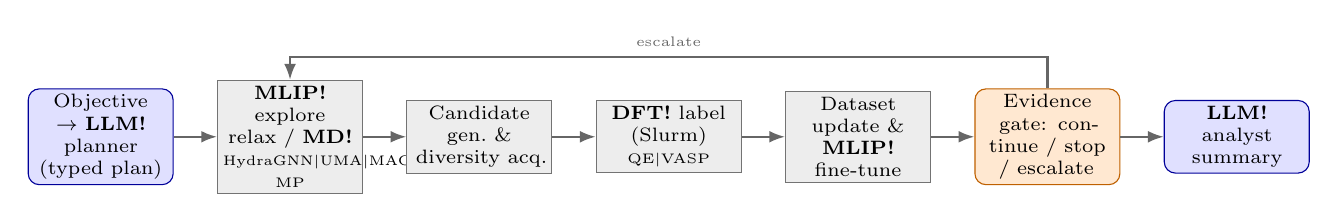
\begin{tikzpicture}[
  node distance=5.5mm,
  font=\scriptsize,
  every node/.style={align=center},
  llm/.style={rectangle, rounded corners, draw=blue!60!black, fill=blue!12,
    text width=17mm, inner sep=2pt, minimum height=9mm},
  det/.style={rectangle, draw=black!55, fill=black!7,
    text width=17mm, inner sep=2pt, minimum height=9mm},
  gate/.style={rectangle, rounded corners, draw=orange!75!black, fill=orange!18,
    text width=17mm, inner sep=2pt, minimum height=9mm},
  arr/.style={-{Latex[length=2mm]}, thick, black!60}
]
\node[llm] (obj) {Objective $\rightarrow$ \acs{LLM} planner (typed plan)};
\node[det, right=of obj] (mlip) {\acs{MLIP} explore relax / \acs{MD}\\{\tiny HydraGNN$\mid$UMA$\mid$MACE-MP}};
\node[det, right=of mlip] (acq) {Candidate gen.\ \& diversity acq.};
\node[det, right=of acq] (dft) {\acs{DFT} label (Slurm) {\tiny QE$\mid$VASP}};
\node[det, right=of dft] (ft) {Dataset update \& \acs{MLIP} fine-tune};
\node[gate, right=of ft] (gate) {Evidence gate: continue / stop / escalate};
\node[llm, right=of gate] (an) {\acs{LLM} analyst summary};
\draw[arr] (obj) -- (mlip);
\draw[arr] (mlip) -- (acq);
\draw[arr] (acq) -- (dft);
\draw[arr] (dft) -- (ft);
\draw[arr] (ft) -- (gate);
\draw[arr] (gate) -- (an);
\draw[arr] (gate.north) -- ++(0,4mm) -| node[pos=0.25, above] {\tiny escalate} (mlip.north);
\end{tikzpicture}
\caption{End-to-end \textsc{matsim-agents} workflow. Blue nodes are
\acs{LLM}-controlled, gray nodes denote explicit scientific-computation stages,
and the orange node is a rule-based gate. LangGraph checkpoints the typed state at
every transition so the loop resumes across batch allocations. All physical
quantities are produced by explicit scientific codes and numerical models rather
than generated by the \acs{LLM}.}
\label{fig:architecture}
\end{figure*}

\subsection{Interface and Orchestration Layer}
The first two layers, the natural-language interface
and the LangGraph orchestration layer, are realized together by a single
multi-agent graph and the entry points that expose it to the user.

\subsubsection{Agent Graph and Nodes}
The agent graph is assembled with LangGraph~\cite{langgraph} and contains four
primary nodes:

\textbf{Planner.} A configurable \ac{LLM} (Qwen2.5-72B via vLLM~\cite{vllm} by
default) turns the user objective into a typed list of \texttt{TaskSpec} items
(\texttt{relax}, \texttt{analyze}, \texttt{report}), using Pydantic schemas for
deterministic \acs{JSON} parsing.

\textbf{Executor.} For each \texttt{relax} task the executor runs \ac{ASE}
\acs{FIRE}/\acs{BFGS} optimisation with the selected \acs{MLIP} backend
(HydraGNN~\cite{hydragnn}, UMA~\cite{wood2025uma}, or
MACE-MP~\cite{batatia2022,batatia2023macemp}) as the force-and-energy evaluator,
appending the optimised structure, final energy, max force, and convergence flag
to the shared typed state.

\textbf{Validation Gate.} After relaxation, a configurable
\emph{post-relaxation gate} decides whether each optimized structure can proceed
to analysis or must be escalated to \acs{DFT}-driven \acs{AL}, based on the
relaxation outcome (convergence and residual forces) and the workflow's
exploration policy. It does not steer the relaxation itself. On acceptance it
passes control to the analyst; otherwise it triggers the \acs{AL} handoff, logging
the decision to a \ac{JSONL} audit file.

\textbf{Analyst.} The analyst node invokes the \acs{LLM} to generate a natural
language summary of the discovered structures, including energy rankings and
stability estimates.

\subsubsection{Entry Points and Task Complexity}
The nodes are exposed through three entry points of increasing scope. The
\emph{default linear graph} handles a single well-posed objective (e.g., ``relax
this structure and report its stability'') in one
planner$\rightarrow$executor$\rightarrow$gate$\rightarrow$analyst pass, the only
branch being escalate-or-summarize. The \emph{supervisor graph} adds a supervisor
over five nodes (prepare, explore, validate, optional \acs{AL}, summarize) that
iterates across a composition space and loops back into \acs{AL} when the gate
flags structures for escalation. The \emph{discovery chat} is an interactive
\ac{REPL} that adds automatic composition detection from free text, optional
multi-\acs{LLM} peer review, and slash commands (\texttt{/relax}, \texttt{/al},
\texttt{/clear}) for human-in-the-loop investigation.

\subsection{Atomistic Backend Layer}
The third layer executes the physics: it evaluates energies and forces with a
configuration-selected \acs{MLIP} backend and escalates flagged structures to
\acs{DFT} through the active-learning and warm-start protocols. Three pretrained
potentials---HydraGNN~\cite{hydragnn,lupopasini2026exascalegfm},
UMA~\cite{wood2025uma}, and MACE-MP~\cite{batatia2022,batatia2023macemp}---sit
behind one calculator interface and are chosen by a single switch
(\texttt{MLIP\_BACKEND}) without touching the orchestration code. HydraGNN is the
default only because it is wired end-to-end on all three platforms; nothing in the
loop, the acquisition step, or the \acs{DFT} interface depends on that choice.

\subsubsection{Pretrained MLIP Backends}
Each backend plugs into the identical calculator, acquisition, and labelling
interfaces; the workflow depends only on their shared contract---energy and force
evaluation orders of magnitude faster than direct \acs{DFT}. The default HydraGNN
\ac{GFM} is an exascale-pretrained multi-task graph model with wide chemical
coverage (architecture and pretraining detailed
in~\cite{lupopasini2026exascalegfm}); UMA~\cite{wood2025uma} and the MACE-MP
models~\cite{batatia2022,batatia2023macemp} are universal potentials used through
their released checkpoints. Any of the three can serve as relaxation engine,
warm-start pre-relaxer, or \acs{AL} starting point.

\subsubsection{Active Learning Loop}
When the validation gate escalates a structure, \textsc{matsim-agents} executes a configurable
number of \acs{AL} iterations. Each iteration proceeds as follows:

\begin{enumerate}
\item \textbf{Candidate generation}: short \ac{MD} trajectories (\acs{ASE} Langevin or
  \ac{NVT}) are run from seed structures to sample configuration space; frames
  whose predicted forces or per-atom displacements exceed physical thresholds
  are discarded, and the survivors are collected as candidates.
\item \textbf{Snapshot selection}: the surviving candidates are down-selected to
  the per-iteration budget using a greedy farthest-point composition-diversity
  filter over configuration descriptors, which removes near-duplicate frames and
  retains geometrically distinct configurations.
\item \textbf{\acs{DFT} labeling}: the top-$n$ selected candidates are submitted
  to the user-selected \acs{DFT} backend (\acs{QE} or \acs{VASP}) as batch jobs,
  and converged frames are written in extended-XYZ format.
\item \textbf{\acs{MLIP} retraining}: the new frames are appended to the training
  set and the selected backend is retrained for a configurable number of epochs
  (HydraGNN from its checkpoint, UMA optionally fine-tuned from its
  foundation-model checkpoint) via a user-supplied training script; when disabled,
  frames are accumulated for offline fine-tuning.
\item \textbf{Loop state serialization}: a \texttt{state.json} per iteration
  records candidate/selection counts, selection statistics, \acs{DFT} convergence rates,
  and timing. Fault-tolerant resume logic skips completed iterations.
\end{enumerate}

The loop is backend-agnostic: the \acs{DFT} interface accepts a
\texttt{DFTJobSpec} and returns converged frames, so \acs{QE} (open source) and
\acs{VASP} (licensed, user-supplied source) are interchangeable from the workflow
perspective.

\subsubsection{DFT Warm-Start Protocol}
A separate warm-start benchmarking module pairs each \acs{MLIP} pre-relaxer
(HydraGNN~\cite{hydragnn} or UMA~\cite{wood2025uma}) with each \acs{DFT} solver
(\acs{QE} via \texttt{warmstart\_benchmark\_qe}, \acs{VASP} via
\texttt{warmstart\_benchmark\_vasp}) as a factorial ablation, so that any
warm-start benefit can be attributed to the potential, the solver, or their
interaction.

The benchmark pipeline, shared across all four configurations, proceeds as follows
for any input crystal structure: (i) an \acs{MLIP} \acs{FIRE} pre-relaxation to
$f_\text{max} = 0.01$\,eV/\AA\ (HydraGNN~\cite{hydragnn} or UMA~\cite{wood2025uma});
(ii) the selected \acs{DFT} solver from the \emph{original} coordinates (cold
start: \acs{QE} \texttt{vc-relax} or the equivalent \acs{VASP} ionic relaxation);
(iii) the same solver from the \emph{\acs{MLIP}-relaxed} coordinates (warm start);
and (iv) comparison of \acs{BFGS} step counts, per-step and total \acs{SCF}
iterations, final energies, and wall times. Identical \acs{DFT} input settings are
used for cold and warm runs to ensure a fair comparison.

% =============================================================================
\section{HPC Deployment}
\label{sec:hpc}

\subsection{Platform-Agnostic Design Principles}
The stack rests on three portability principles. \textbf{Module isolation:} all
\acs{GPU}-software interactions (\acs{CUDA}/\acs{MPI}/compiler toolchain) are
encapsulated behind per-platform shell fragments, so a single function
(\texttt{load\_perlmutter\_modules\_gpu()} or its Frontier/Aurora equivalents)
sets up the whole environment reproducibly from a clean login shell.
\textbf{Decoupled Python and \ac{MPI} environments:} the \acs{MLIP} backends run
in a PyTorch \acs{GPU} environment while \acs{QE}/\acs{VASP} need separate
\acs{MPI}/compiler stacks, so the batch script activates the Python environment
for the \acs{MLIP} phase and spawns the \acs{DFT} launcher as a subprocess with
its own compiler/\acs{MPI}/runtime. \textbf{vLLM inference serving:} \acs{LLM}
inference runs in a separate Slurm allocation (or a login-node background process)
behind an OpenAI-compatible \ac{HTTP} endpoint, requiring only the \texttt{openai}
package on the client side. The first-principles code is exposed as a
user-selectable backend (\acs{QE} or \acs{VASP}); the repository ships build and
launch scripts for both on Perlmutter, Frontier, and Aurora, documenting the
module loads, compiler choices, \acs{MPI}/offload settings, and launcher
conventions each system requires, while \acs{VASP} users must supply their own
licensed source and pseudopotentials.

\subsection{Per-Platform Deployment}
The framework is built and deployed on all three \acs{DOE} leadership-class
systems, each with a distinct accelerator and \acs{DFT} offload backend
(Perlmutter/NVIDIA A100 via NVHPC \acs{CUDA}, Frontier/AMD MI250X via HIP OpenMP
target offload, Aurora/Intel \acs{PVC} via OneAPI); the per-platform module
loads, compiler choices, and offload settings live in the released build scripts.


% =============================================================================
\section{Experimental Results}
\label{sec:results}

All experiments in this section were run on \acs{NERSC} Perlmutter. The warm-start
and fine-tuning studies use a single compute node (4$\times$ NVIDIA A100 80\,GB);
the end-to-end campaigns and the strong-scaling study use one to eight such nodes,
as noted in each table.

\subsection{Warm-Start Benchmark Setup}
\label{sec:results:warmstart_setup}
The warm-start benchmarks are organized as a controlled comparison between two
ways of initializing each first-principles geometry optimization:

\begin{itemize}
\item \textbf{Cold start.} The \acs{DFT} optimizer is launched directly from the
  \emph{original} input coordinates of the fixture, with no \acs{MLIP}
  pre-processing. This is the conventional baseline.
\item \textbf{Warm start.} The same fixture is first relaxed by an \acs{MLIP}
  to $f_\text{max} = 0.01$\,eV/\AA, and the \acs{DFT} optimizer is then launched
  from the \emph{\acs{MLIP}-relaxed} coordinates. The \acs{DFT} settings are held
  identical to the cold run so that any difference in convergence is
  attributable solely to the change of initial geometry.
\end{itemize}

The cold/warm pair is repeated for all four combinations of \acs{MLIP}
pre-relaxer (HydraGNN~\cite{hydragnn} or UMA~\cite{wood2025uma}) and \acs{DFT}
solver (\acs{QE} or \acs{VASP}), a factorial ablation in which varying one factor
at a time attributes any warm-start benefit to the potential, the solver, or
their interaction. Three off-equilibrium alloy fixtures are used---MoNbTaW
\acs{HEA} (16-atom BCC), NbTaW BCC, and NbMoW BCC---each run three times per
backend pairing on Perlmutter; the recorded quantities are the \acs{BFGS}
ionic-step count, per-step and total \acs{SCF} iterations, final energy, and wall
time.

\subsection{Warm-Start across All Backend Pairings: Alloy Fixtures}
\label{sec:results:warmstart_hea}
The three alloy fixtures---MoNbTaW \acs{HEA} (16-atom BCC), NbTaW BCC, and NbMoW
BCC---have random site occupation, so the input geometry carries genuine
site-specific forces and the \acs{MLIP} pre-relaxation moves atoms before
converging. Each fixture is run under all four backend pairings, giving the
twelve rows of Table~\ref{tab:warmstart_matrix}. Each row reports the \acs{BFGS}
ionic-step count and total \acs{SCF} iteration count for the cold and warm runs
(averaged over three repeats) and the relative change in total \acs{SCF} work,
$\Delta_\text{SCF} = (\text{warm}-\text{cold})/\text{cold}$, where negative values
indicate a warm-start speed-up. Varying one backend factor at a time isolates
whether any benefit comes from the \acs{MLIP} pre-relaxer or the \acs{DFT} solver.

\begin{table*}[tp]
\centering
\caption{Cold vs.\ warm-start convergence for the factorial backend ablation
across the three alloy fixtures.}
\label{tab:warmstart_matrix}
\begin{tabular}{lllcccccc}
\toprule
\multirow{2}{*}{Fixture} & \multirow{2}{*}{\acs{MLIP}} & \multirow{2}{*}{\acs{DFT}}
 & \multicolumn{2}{c}{\acs{BFGS} steps} & \multicolumn{2}{c}{Total \acs{SCF}} & \multirow{2}{*}{$\Delta_\text{SCF}$} & \multirow{2}{*}{Repeats}\\
\cmidrule(lr){4-5}\cmidrule(lr){6-7}
 & & & Cold & Warm & Cold & Warm & & \\
\midrule
\multirow{4}{*}{MoNbTaW \acs{HEA}} & HydraGNN & \acs{QE} & 5 & 5 & 127 & 127 & 0\% & 3 \\
 & HydraGNN & \acs{VASP} & 7 & 7 & 75 & 75 & 0\% & 3 \\
 & UMA & \acs{QE} & 5 & 5 & 127 & 143 & +13\% & 3 \\
 & UMA & \acs{VASP} & 7 & 7 & 75 & 74 & $-$1\% & 3 \\
\cmidrule(lr){1-9}
\multirow{4}{*}{NbTaW BCC} & HydraGNN & \acs{QE} & 5 & 2 & 134 & 224.7 & +68\% & 3 \\
 & HydraGNN & \acs{VASP} & 6 & 6 & 61 & 61 & 0\% & 3 \\
 & UMA & \acs{QE} & 5 & 4 & 134 & 109 & $-$19\% & 3 \\
 & UMA & \acs{VASP} & 6 & 6 & 61 & 56 & $-$8\% & 3 \\
\cmidrule(lr){1-9}
\multirow{4}{*}{NbMoW BCC} & HydraGNN & \acs{QE} & 6 & 6 & 158.3 & 158 & 0\% & 3 \\
 & HydraGNN & \acs{VASP} & 8 & 8 & 76 & 76 & 0\% & 3 \\
 & UMA & \acs{QE} & 6 & 5 & 158 & 141 & $-$11\% & 3 \\
 & UMA & \acs{VASP} & 8 & 5 & 76 & 48 & $-$37\% & 3 \\
\bottomrule
\end{tabular}
\end{table*}

The completed matrix shows a backend-dependent split. On the disordered \acs{BCC}
alloys, UMA-relaxed geometries reduce total \acs{DFT} \acs{SCF} work across
\emph{both} solvers---UMA+\acs{QE} by $19\%$ (NbTaW) and $11\%$ (NbMoW), and
UMA+\acs{VASP} by $8\%$ (NbTaW) and $37\%$ (NbMoW)---whereas HydraGNN
pre-relaxation is neutral on \acs{VASP} ($0\%$ on all three fixtures) and, on
NbTaW+\acs{QE}, \emph{increases} cost ($\Delta_\text{SCF}=+68\%$, with the warm
run exhausting its \acs{SCF} budget without converging). These results show that warm-start behavior depends on both the material and the
backend. A change in \acs{SCF} work reflects not only the quality of the
pre-relaxed geometry but also solver conditioning and pseudopotential choice, so
the results should not be interpreted as a universal ranking of potentials.
Instead, \acs{MLIP} pre-relaxation can reduce \acs{DFT} optimization effort for
some material--backend combinations and increase it for others; its benefit
should therefore be evaluated for the target workflow. Because the backend is a user-selectable
configuration rather than a hard-coded dependency, the same run can switch or
benchmark potentials on identical fixtures without changing the agentic
orchestration, the \acs{DFT} escalation logic, or the deployment scripts.

\subsection{End-to-End Integration and Throughput}
\label{sec:results:al}
The central systems claim of \textsc{matsim-agents} is that its components---
seed generation, \acs{MLIP}-driven \acs{MD} sampling, candidate
acquisition, \acs{DFT} labelling, dataset assembly, and model
retraining---compose into a single automated loop that runs unattended on
leadership \acs{HPC}. To validate this we executed the \acs{AL} loop
end to end on all five cases for five distinct classes of compounds, on \acs{NERSC} Perlmutter using the OpenACC
\acs{GPU} build of
\acs{VASP}~6.6.0 on NVIDIA A100 nodes. Each iteration proceeds without human
intervention: seeds are propagated by short Langevin \acs{MD} (400 steps,
2\,fs, 1000\,K) under the \acs{MLIP} force engine; snapshots are sub-sampled
every 15 steps and screened by force and displacement thresholds; the surviving
candidates are down-selected under a per-iteration
budget with a composition-diversity filter; the selected frames are labelled by
concurrent single-point \acs{VASP} jobs; and the converged frames are appended
to the growing training set. State is checkpointed per iteration so runs resume
after walltime limits.

The performance is tested on five classes of compounds that span diverse chemical classes and dimensionalities:
LiFePO\textsubscript{4} olivine (3D battery cathode), NbTaVHfZrTi \acs{BCC} and
CrMnFeCoNi Cantor FCC \acsp{HEA} (3D refractory and structural alloys),
phosphorene (2D semiconductor), and the Zn(HCOO)\textsubscript{2} \acs{MOF} (3D
porous framework).

The single-point \acs{DFT} settings used to label every frame are summarized in
Table~\ref{tab:dft}. All systems share a single, internally consistent
Perdew--Burke--Ernzerhof (PBE) generalized-gradient exchange--correlation
functional with projector augmented-wave (PAW) potentials, so that the surrogate
learns from one uniform reference across chemistries; per-case choices vary only
in spin treatment, smearing, and k-point density. The magnetic $3d$ systems
(LiFePO\textsubscript{4} and the CrMnFeCoNi Cantor alloy) are computed
spin-polarized (\texttt{ISPIN}$=2$); no Hubbard $+U$ correction is applied to any
system, so the LiFePO\textsubscript{4} reference is spin-polarized plain
\acs{GGA}. We deliberately keep a single uniform functional across all five
chemistries because the object of study is the orchestration workflow and the
surrogate's ability to reproduce its own \acs{DFT} target, not the absolute
electrochemical accuracy of any one material; a $+U$ or hybrid reference for the
Fe-$3d$ states would improve LiFePO\textsubscript{4} redox energetics but is
orthogonal to the workflow claims and is left to future work.

\begin{table}[tb]
\centering
\caption{Per-case single-point \acs{VASP}/PAW settings. Shared across all cases:
PBE (\acs{GGA}) functional, \texttt{ENCUT}$=520$\,eV, \texttt{EDIFF}$=10^{-6}$\,eV,
$\Gamma$-centred k-meshes, \texttt{NSW}$=0$, and no Hubbard $+U$.}
\label{tab:dft}
\footnotesize
\setlength{\tabcolsep}{4pt}
\resizebox{\columnwidth}{!}{%
\begin{tabular}{lccc}
\toprule
System & Spin (\texttt{ISPIN}) & Smearing ($\sigma$/eV) & \texttt{KSPACING} (\AA$^{-1}$)\\
\midrule
LiFePO\textsubscript{4} olivine     & polarized (2)   & Gaussian (0.05) & 0.30 \\
CrMnFeCoNi Cantor FCC \acs{HEA}     & polarized (2)   & MP-1 (0.20)     & 0.22 \\
NbTaVHfZrTi BCC \acs{HEA}           & unpolarized (1) & MP-1 (0.20)     & 0.25 \\
Phosphorene (black-P)               & unpolarized (1) & Gaussian (0.05) & 0.25 \\
Zn(HCOO)\textsubscript{2} \acs{MOF} & unpolarized (1) & Gaussian (0.05) & 0.30 \\
\bottomrule
\end{tabular}%
}
\end{table}

Table~\ref{tab:al} reports per-case throughput---completed iterations, total
\acs{MD} candidates, candidates selected for labelling, converged and failed
single-point \acs{VASP} jobs, and cumulative \acs{DFT} labelling wall time.
Across all cases the loop executed
the full pipeline without manual intervention, dispatching \acs{DFT} jobs concurrently within a
four-node allocation (four one-node \acs{VASP} jobs at a time, or two two-node
jobs for the denser Zn(HCOO)\textsubscript{2} framework), and recovering
automatically across the checkpoint boundary. \acs{DFT} convergence rates were
high (\(>94\%\) in every case, and \(100\%\) for phosphorene and
LiFePO\textsubscript{4}), confirming that the \acs{MD} screening stage supplies
physically reasonable structures to \acs{VASP}.

\begin{table}[tb]
\centering
\caption{End-to-end \acs{AL} throughput on Perlmutter, four A100 nodes per case.}
\label{tab:al}
\resizebox{\columnwidth}{!}{%
\begin{tabular}{lccccccc}
\toprule
System & Nodes & Iters & Cand. & Sel. & Conv. & Fail & \acs{DFT} wall (h)\\
\midrule
Phosphorene (black/blue-P)          & 4 & 8  & 160  & 160  & 160 & 0  & 2.60 \\
LiFePO\textsubscript{4} olivine     & 4 & 10 & 144  & 144  & 144 & 0  & 5.04 \\
CrMnFeCoNi Cantor FCC \acs{HEA}     & 4 & 12 & 433  & 433  & 432 & 1  & 6.17 \\
NbTaVHfZrTi BCC \acs{HEA} & 4 & 5  & 1650 & 1000 & 942 & 58 & 8.42 \\
Zn(HCOO)\textsubscript{2} \acs{MOF} & 4 & 4 & 32 & 32 & 32 & 0 & 0.61 \\
\bottomrule
\end{tabular}%
}
\end{table}

\begin{figure}[tb]
\centering
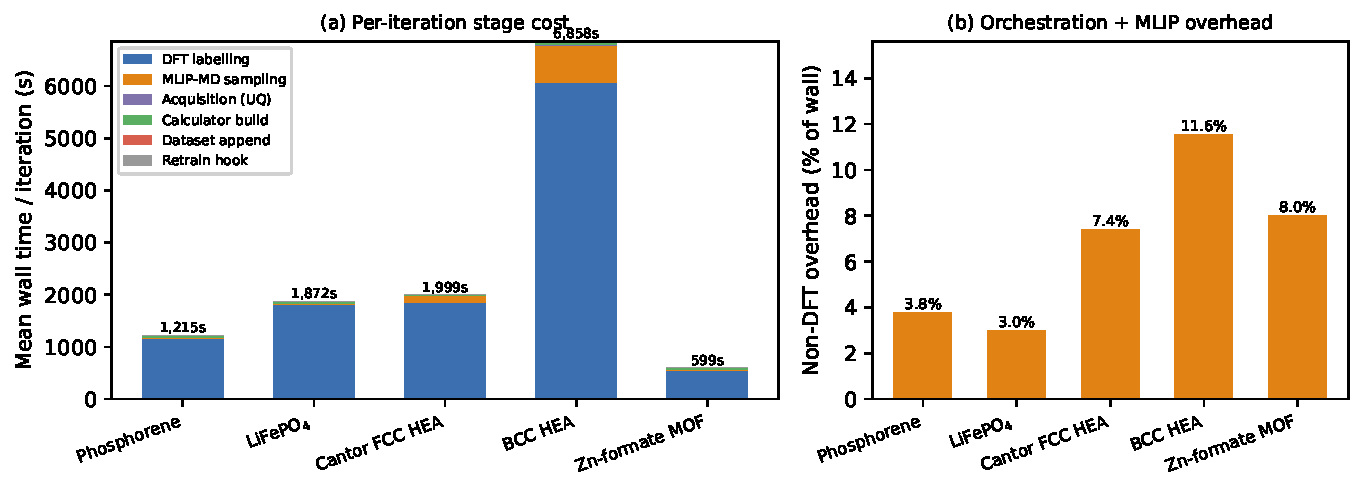
\includegraphics[width=\columnwidth]{figures/al_timing_breakdown.pdf}
\caption{Per-iteration wall-time breakdown of the \acs{AL} loop across
the five cases covering five distinct classes of compounds. (a) Mean wall time per iteration, stacked by stage.
(b) Combined non-\acs{DFT} time (calculator construction, \acs{MLIP}-\acs{MD}
sampling, candidate acquisition, dataset append, and the retrain hook) as a
percentage of iteration wall time.}
\label{fig:al_timing}
\end{figure}

Figure~\ref{fig:al_timing} decomposes the per-iteration wall time by stage.
Single-point \acs{DFT} labelling accounts for 88--97\% of the wall clock in
every case, while all non-\acs{DFT} stages combined---building the
\acs{MLIP} calculator, running the Langevin \acs{MD} sampler, selecting
candidates by the composition-diversity filter, appending the labelled frames, and invoking the
retrain hook---contribute only 3--12\%. These figures bound the aggregate
non-\acs{DFT} cost; they do not separately quantify \acs{LLM} inference, LangGraph
transitions, state serialization, or scheduler interaction, which we do not
measure individually. The acquisition and dataset-management
stages are sub-second to a few seconds per iteration (e.g.\ 2.6\,s acquisition
and 0.15\,s append for the Cantor \acs{HEA}); the only non-trivial non-DFT cost
is \acs{MLIP}-\acs{MD} sampling, which scales with system size and step count.
The aggregate non-\acs{DFT} cost remains small relative to first-principles
labelling, so \acs{DFT} remains the dominant computational cost of the workflow.

The loop is also resilient to the wall-clock limits that dominate shared
\acs{HPC} scheduling. State is checkpointed after every iteration (a
per-iteration \texttt{state.json} plus the growing \texttt{dataset.extxyz}), so
a job that is pre-empted or hits its wall-time limit resumes from the last
completed iteration on resubmission with no manual bookkeeping. The
LiFePO\textsubscript{4} run in Table~\ref{tab:al}, for instance, was interrupted
by a wall-time limit after five iterations and completed the remaining five in a
second allocation, reusing every previously labelled frame. This
checkpoint-and-resume behaviour lets long campaigns span many short,
backfill-friendly allocations rather than requiring a single monolithic
reservation.

We highlight that, for four of the five cases, the number of screened
\acs{MD} candidates fell at or below the per-iteration budget, so essentially
every valid frame was labelled; the BCC \acs{HEA} is the exception, generating
more candidates (1650) than its budget (1000 selected), so the
composition-diversity filter actively down-selected. Accordingly, these experiments establish end-to-end integration and throughput
rather than sample-efficiency gains from the acquisition strategy. In-loop
retraining is exercised, while systematic comparison of acquisition strategies
is left to future work.

\subsection{Fine-Tuning on Active-Learning-Corrected Data}
\label{sec:results:finetune}
The end-to-end loop of Section~\ref{sec:results:al} produces, for each paper
case, a compact set of \acs{DFT}-labelled frames drawn precisely from the
configurations the \acs{MLIP} itself sampled during \acs{MD}. We next evaluate whether retraining the force engine on the resulting
\acs{DFT}-labelled data improves accuracy for the corresponding chemistry. We
therefore ran a controlled \emph{fine-tune-and-evaluate} study on all five cases,
using the per-case datasets accumulated by the loop
(LiFePO\textsubscript{4}, Cantor FCC \acs{HEA}, NbTaVHfZrTi BCC \acs{HEA},
phosphorene, and the Zn(HCOO)\textsubscript{2} \acs{MOF}).

\paragraph{Protocol}
Each per-case dataset is divided into disjoint train and held-out test partitions
by a single random frame-level $80/20$ split (fixed seed $0$, one draw per case;
no separate validation partition). The total/train/test frame counts and number of \acs{AL} iterations are
$29/23/6$ ($10$) for LiFePO\textsubscript{4}, $86/69/17$ ($12$) for Cantor FCC,
$434/347/87$ ($5$) for NbTaVHfZrTi BCC, $32/26/6$ ($8$) for phosphorene, and
$13/10/3$ ($4$) for the Zn(HCOO)\textsubscript{2} \acs{MOF}. Given its
three-frame held-out partition, the \acs{MOF} result is treated as illustrative
rather than as a basis for cross-backend comparison. The study is intended to
measure model adaptation on loop-generated data rather than to establish
large-data benchmark rankings. We measure a strict
\emph{before/after} pair on the identical test partition: the \emph{before}
endpoint is the pretrained checkpoint with no exposure to the case data, and the
\emph{after} endpoint is the same architecture fine-tuned on the train partition.
We report two error metrics per endpoint: the force mean absolute error
(\acs{MAE}, eV/\AA) and the per-atom energy \acs{MAE} after subtracting a
per-element linear reference (meV/atom). The frame-level split is used consistently across all backends. Because
neighboring \acs{MD} frames can be temporally correlated, the resulting metrics
characterize within-trajectory held-out performance; future evaluations will also
use trajectory- or iteration-level partitions. In the current implementation the
per-element linear reference for the shifted energy metric is fit on the held-out
frames. We therefore mark the reference-shifted energy \acs{MAE} and use force \acs{MAE}, 
which is unaffected by that reference fit, as the
principal fine-tuning metric. A training-partition reference will be used in the
next evaluation. Each campaign is run once with a fixed seed, so the table reports
point estimates.

\paragraph{Backends}
The study spans all three \acs{MLIP} engines used elsewhere in the paper. For
HydraGNN~\cite{hydragnn} we contrast four transfer-learning strategies against a
common baseline: (i) \emph{routed}, the default multi-head \ac{GFM} routing;
(ii) \emph{unfrozen}, a full fine-tune of the backbone and heads; (iii)
\emph{frozen}, in which the backbone is held fixed and only the output head is
retrained; and (iv) \emph{scratch}, a model trained from random initialization
on the case data alone, which isolates the value of the pretrained
representation. For UMA~\cite{wood2025uma} we fine-tune directly through the
model's conservative energy-and-force head with a custom training
loop, a small number of Adam epochs on a force-weighted energy-and-force loss
that updates the pretrained output heads in place, in three variants:
\emph{full} (all trainable weights), \emph{frozen} (backbone held fixed, output
head only), and \emph{LoRA}, in which low-rank adapters are inserted into the
backbone's scalar and radial linear layers, leaving the equivariant tensor
operations untouched. For MACE~\cite{batatia2022,batatia2023macemp} we fine-tune
the released MACE-MP foundation models at all three published capacities
(\emph{small}, \emph{medium}, \emph{large}) using the authors' own training
entry point, in two variants: a \emph{naive} full fine-tune and a native
\emph{LoRA} fine-tune. All fine-tunes adapt the pretrained potential to a narrow
domain, and every backend is scored on the same held-out partition with the same
metrics, so the comparison is on common data partitions and evaluation metrics
rather than identical training conditions (optimizers, trainable-parameter counts,
budgets, and implementations differ across backends).

\paragraph{Fine-tuning through the conservative force head}
UMA is a \emph{conservative} potential: it predicts one energy and takes the
forces as the exact gradient of that energy, keeping energies and forces
consistent. For these datasets, directly applying the default fine-tuning procedure produced
two undesirable effects. Recomputing the energy/force normalization scales from
the case data increased the force scale by about $3\times$, and replacing the
conservative head with a \emph{direct}-force head removed the energy-gradient
constraint. We therefore fine-tune the original conservative head while retaining
the pretrained normalization scales. In our tests, refitting the normalizer on
the case-specific data degraded accuracy without producing an explicit runtime
error.

\paragraph{Cross-backend results}
Figure~\ref{fig:finetune} reports the held-out force \acs{MAE} (principal metric)
and the reference-shifted energy \acs{MAE} for every backend
and fine-tuning variant on the five \acs{AL}-corrected cases for five distinct classes of compounds, each grouped
under its zero-shot baseline. Because all methods are scored on the same held-out
frames with the
same metrics, the figure compares HydraGNN, UMA, and the three MACE-MP capacities
on common data partitions and evaluation metrics (training conditions differ
across backends). The zero-shot errors indicate limited transfer to several of
these specialized chemistries (battery cathode, refractory and structural
\acsp{HEA}, 2D semiconductor, porous \acs{MOF}), regardless of whether related
configurations appeared in the original pretraining corpora. Fine-tuning on the
loop-generated data reduces one or both error metrics for many backend--material
combinations, but neutral and negative transfer also occurs and is a meaningful
outcome rather than an exception.

For HydraGNN the full (\emph{unfrozen}) fine-tune and the from-\emph{scratch}
specialist give the largest, similar reductions, while the head-only
(\emph{frozen}) and default \emph{routed} updates change the metrics least; the
competitiveness of the from-scratch model suggests the \acs{AL}-corrected
datasets are internally consistent. For UMA the figure contrasts full fine-tuning
with parameter-efficient variants (head-only and LoRA), and for the MACE-MP
capacities naive full fine-tuning with LoRA, using the authors' native training
entry point. These results compare backend behavior under a common evaluation protocol rather
than define a universal ranking: the lowest-error backend and adaptation strategy
depend on the material and metric. The uniform interface lets a user switch
or benchmark potentials on identical held-out frames, so the choice of potential
remains the user's, per material and per task.

\begin{figure*}[tp]
\centering
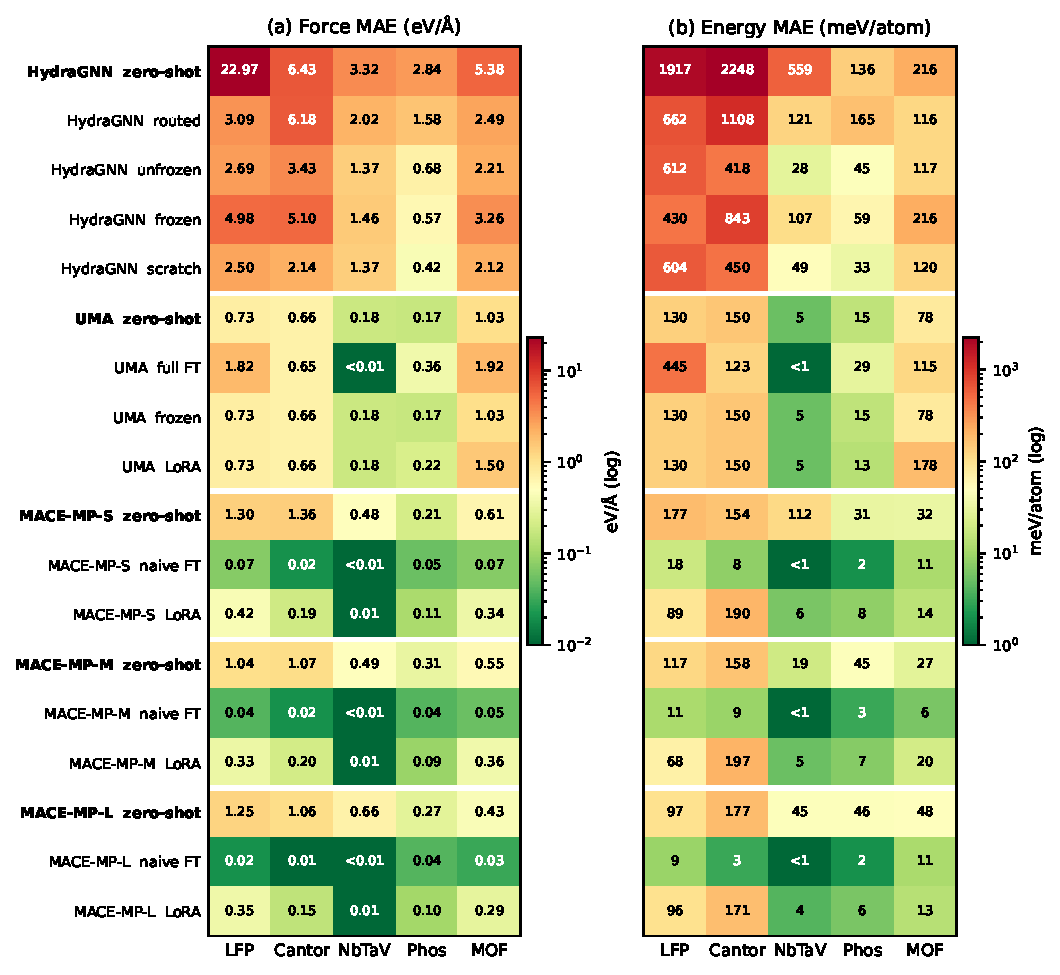
\includegraphics[width=0.66\textwidth]{figures/finetune_matrix.pdf}
\caption{Held-out test errors on the \acs{AL}-corrected cases, unified
across all three \acs{MLIP} backends and their fine-tuning variants.
(a)~force \acs{MAE} (eV/\AA); (b) reference-shifted per-atom
energy \acs{MAE} (meV/atom; elemental reference fit on the test frames, see
Section~\ref{sec:conclusions}). Rows are grouped by backend, each backend's
zero-shot baseline
(bold) followed by its fine-tuning variants; case columns are LFP
(LiFePO\textsubscript{4}), Cantor, NbTaV (NbTaVHfZrTi), Phos (phosphorene), and
MOF (Zn(HCOO)\textsubscript{2}); MACE-MP S/M/L $=$ small/medium/large.
Colour is log-scaled (green $=$ low error, red $=$ high error), so the
order-of-magnitude drop from zero-shot to fine-tuned is visible at a glance
while every cell is annotated with its exact value.}
\label{fig:finetune}
\end{figure*}


\subsection{Evidence-Gated Escalation}
\label{sec:results:hypothesis}
The fine-tuning results quantify \emph{how accurate} each surrogate is; this
subsection shows how that accuracy sets the workflow's \emph{recommended
action}---continue surrogate screening or escalate to \acs{DFT}. Through the
discovery-chat entry point (Section~\ref{sec:architecture}) a user types a single
free-text objective---for the Cantor alloy, for instance, to decide which of
FCC/BCC/HCP is simultaneously chemically and dynamically stable and to give the
numerical criterion that would falsify the claim. The workflow auto-detects the
composition, enumerates the candidate polymorphs, and hands them to an optional
multi-\acs{LLM} panel: a proposer (Qwen2.5-14B-Instruct) and two critics from
independent developers (DeepSeek-R1-Distill-Qwen-32B and Gemma~4~31B), served
locally through vLLM. The panel's only surrogate evidence is the measured
held-out accuracy of Fig.~\ref{fig:finetune}, so any change in its recommended
action is a function of the reported numbers alone.

We run three fixtures---the two \acs{HEA}s and the LiFePO$_4$
cathode---under two evidence conditions: zero-shot (\emph{before}) and fine-tuned
(\emph{after}). A rule-based gate encodes the rule the panel is asked to
respect: if the best available force \acs{MAE} exceeds the
$\sim\!0.005$\,eV/\AA\ needed to trust phonon signs (and the coarser resolution
needed to separate competing polymorphs), escalate to \acs{DFT} and route the
structures back into \acs{AL}; otherwise permit surrogate screening subject to
\acs{DFT} validation. We drive the gate on the force \acs{MAE}, our principal and
leakage-free metric, and deliberately exclude the reference-shifted energy
\acs{MAE}, whose elemental reference is fit on the test frames
(Section~\ref{sec:conclusions}). Table~\ref{tab:hypothesis} shows the recommended
action tracking the gate: before fine-tuning the best force \acs{MAE} is
$0.18$--$0.73$\,eV/\AA\ and the panel escalates, whereas after fine-tuning it
falls to $\le\!0.01$\,eV/\AA\ on the \acsp{HEA} (screening permitted subject to
\acs{DFT} validation) while LiFePO$_4$ remains at $0.02$\,eV/\AA---still too
coarse for phonon signs---so \acs{DFT} is required. The before/after evidence also
surfaces cases where fine-tuning \emph{degrades} a universal potential (UMA and
HydraGNN regress on LiFePO$_4$).

An aggregate held-out \acs{MAE} does not certify the phase
stability of any specific candidate, nor is it a candidate-specific uncertainty;
it only bounds how finely the surrogate can discriminate, which is what the gate
needs. The \acs{LLM} panel interprets the reported evidence in natural language,
but the rule-based gate makes the escalate/permit decision and every stability
conclusion still requires \acs{DFT}. Thus, measured surrogate quality determines whether the workflow continues with
surrogate screening or invokes first-principles evaluation.

\begin{table}[tb]
\centering
\footnotesize
\caption{Evidence-gated recommended actions before vs.\ after \acs{AL}
fine-tuning. All three fixtures share one user objective (decide the stable
structure and give a falsification criterion); only the element set differs.
``Min.\ force \acs{MAE}'' is the smallest held-out force error over the three
backends (Fig.~\ref{fig:finetune}).}
\label{tab:hypothesis}
\setlength{\tabcolsep}{5pt}
\begin{tabular}{lccl}
\toprule
Fixture & \shortstack{Before\\(eV/\AA)} & \shortstack{After\\(eV/\AA)} & Recommended action\\
\midrule
Cantor FCC & 0.66 & 0.01 & Escalate $\rightarrow$ screen, then \acs{DFT} validate\\
NbTaV BCC  & 0.18 & $<$0.01 & Escalate $\rightarrow$ screen, then \acs{DFT} validate\\
LiFePO$_4$ & 0.73 & 0.02 & Escalate $\rightarrow$ \acs{DFT} required (phonons)\\
\bottomrule
\end{tabular}
\end{table}

\subsection{Strong Scaling of DFT Labeling}
\label{sec:results:scaling}
The per-iteration breakdown of Fig.~\ref{fig:al_timing} shows that
single-point \acs{DFT} labelling accounts for 88--97\% of the loop's wall time,
which raises a natural systems question: how does that dominant stage respond
to additional node allocation? To answer it we ran a controlled strong-scaling
study in which a \emph{fixed} 32-frame workload of FCC \acs{HEA}
configurations, drawn from CrMnFeCoNi and four near-equimolar FCC
compositions, is labelled by single-point \acs{VASP} at four node counts,
$N\in\{1,2,4,8\}$. Concurrency is expressed as $N$ simultaneous one-node
\acs{VASP} jobs (four A100 ranks each), so $N$ nodes process the same 32 frames
with $N$-way parallelism. Because the workload is held fixed while the resource
grows, this is a strong-scaling (fixed-problem) measurement.

To make the result defensible against per-draw variability we repeat the sweep
$R=5$ times, each drawing an independent random 32-frame workload held fixed
across node counts within the repeat. Throughput is measured from in-job timers
as converged frames per \acs{DFT}-hour
($\text{throughput} = n_\text{conv}/t_\text{DFT}\times 3600$), independent of
scheduling latency, and parallel efficiency is
$100\times(\text{throughput}_N/N)/\text{throughput}_1$ relative to the single-node
baseline.

\begin{figure}[tb]
\centering
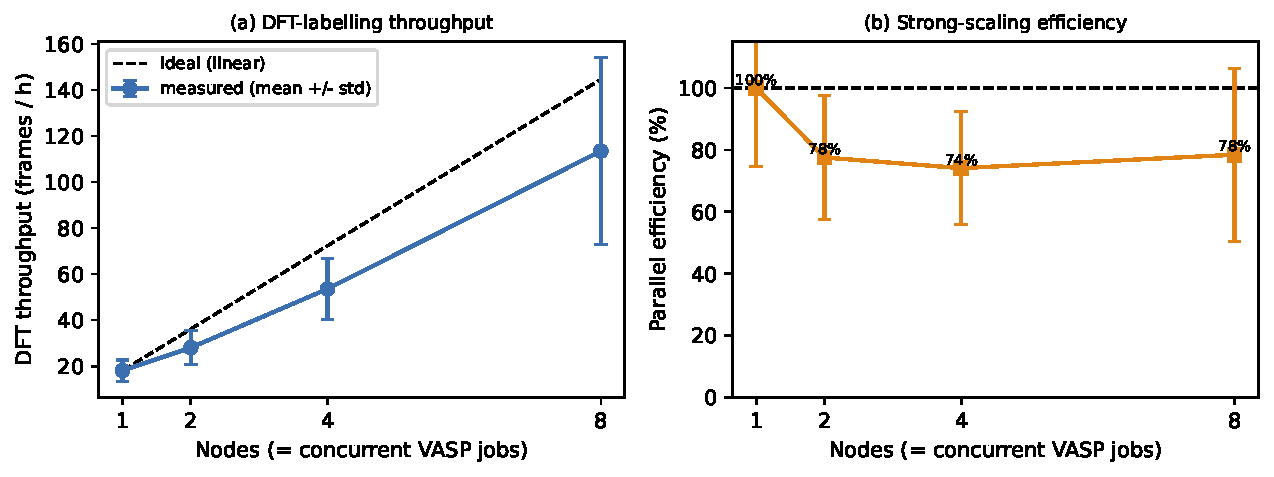
\includegraphics[width=\columnwidth]{figures/al_dft_scaling.pdf}
\caption{Strong scaling of the \acs{DFT}-labelling stage on Perlmutter: a fixed
32-frame FCC \acs{HEA} workload labelled with $N$-way single-point \acs{VASP}
concurrency ($N\in\{1,2,4,8\}$ one-node jobs, four A100 ranks each).
(a) Work-normalized \acs{DFT} throughput (converged frames per \acs{DFT}-hour)
and (b) parallel efficiency vs.\ node count, each averaged over $R=5$ randomized
workload draws with $\pm$ one standard deviation error bars; the dashed line is
the ideal-linear reference.}
\label{fig:al_dft_scaling}
\end{figure}

Figure~\ref{fig:al_dft_scaling} reports the mean throughput and parallel
efficiency over the five repeats. Throughput rises from $18.1\pm4.6$ frames/h on
one node to $28.0\pm7.3$ (two nodes), $53.6\pm13.3$ (four nodes), and
$113.5\pm40.5$ (eight nodes), corresponding to speedups of $1.55\times$,
$2.96\times$, and $6.28\times$. Parallel efficiency remains between 74\% and
79\% across the scaled runs.

The residual sublinear scaling is a property of the \emph{fixed} workload rather
than the resource: random alloy frames differ widely in \acs{SCF}
difficulty, so at high concurrency the makespan is set by the slowest frame in a
repeat (enlarging the workload from $16$ to $32$ frames raises eight-node
throughput from $66.9$ to $113.5$ frames/h). The embarrassingly parallel
\acs{DFT}-labelling workload thus retains approximately $74$--$79\%$ parallel
efficiency up to eight concurrent nodes; production runs should match the node
allocation to the acquisition-batch size. This experiment measures labelling
throughput and does not separately quantify scheduler latency.

\subsection{Backend and Platform Portability of the Loop}
\label{sec:results:portability}
The loop treats both the \acs{MLIP} and the first-principles engine as
configuration-selected backends rather than hard-coded dependencies, so the same
orchestration targets different accelerators and \acs{DFT} codes without code
changes. On Perlmutter the identical phosphorene loop labels structures with
either \acs{VASP} or \acs{QE} by changing only the \texttt{dft:} block of the
configuration; each code is reached through a thin per-platform launcher that
performs its own module swap, so the driver's Python/\acs{MLIP} environment never
collides with the \acs{DFT} code's compiler/\acs{MPI} stack. HydraGNN builds on
all three target accelerators and both \acs{QE} and \acs{VASP} compile on all
three facilities (Section~\ref{sec:hpc}), but end-to-end campaigns with reported
measurements are illustrated only on Perlmutter; the
framework is thus portable by design, with performance illustrated on one
platform.

% =============================================================================
\section{Conclusions and Future Work}
\label{sec:conclusions}

We presented \textsc{matsim-agents}, an open-source agentic workflow that connects
natural-language scientific objectives to \acs{MLIP}-based exploration,
first-principles labeling, model adaptation, and evidence-based escalation on
leadership-class \acs{HPC}. The system separates orchestration from the scientific
backends, checkpoints workflow state across batch allocations, and allows the
\acs{MLIP} and \acs{DFT} engines to be selected through configuration rather than
hard-coded into the workflow. On Perlmutter, five end-to-end campaigns ran without
manual intervention and resumed across allocation boundaries. Across these
campaigns, single-point \acs{DFT} labeling accounted for $88$--$97\%$ of iteration
wall time, while all non-\acs{DFT} stages combined accounted for $3$--$12\%$.
The dominant labeling stage retained approximately $74$--$79\%$ parallel
efficiency from one to eight concurrent nodes.

The experiments also show that the usefulness of surrogate models depends on the
material, backend, and task. \acs{MLIP} pre-relaxation reduced \acs{DFT} effort for
several material--backend combinations but was neutral or detrimental for others.
Likewise, fine-tuning improved many backend--material combinations but did not
produce a uniform benefit. These results motivate the backend abstraction used in
\textsc{matsim-agents}: model selection and adaptation are treated as workflow
choices informed by measured performance rather than as fixed assumptions. The
escalation experiment follows the same principle by using measured
force error to determine when surrogate screening is appropriate and when the
workflow should invoke \acs{DFT}.

The present study focuses on demonstrating integrated execution, portability of
the software design, and model adaptation on loop-generated data. The
fine-tuning analysis uses frame-level held-out splits, so future evaluations will
add trajectory- and iteration-level partitions to quantify transfer across less
correlated configurations.
Systematic comparisons of the acquisition strategy against random, uniform, and
uncertainty-based selection will also be used to quantify sample efficiency.

Future work will extend the perform end-to-end campaigns beyond Perlmutter
to Frontier and Aurora, expand in-loop adaptation across additional \acs{MLIP}
backends, and introduce intermediate-fidelity models such as \ac{DFTB}+ where they
can reduce the number of full \acs{DFT} evaluations. Additional literature and
materials-database tools will broaden the information available to the planning
layer. These developments will move the framework from the present focus on
stability characterization toward broader materials-discovery workflows while
retaining the same separation between language-model orchestration and explicit
scientific computation.

% =============================================================================
\section*{Acknowledgments}
This work was primarily supported by the Office of Advanced Scientific Computing Research (ASCR) and Office of Basic Energy Sciences through the SciDAC project ``FORUM-AI: Foundation Models Orchestrating Reasoning Agents to Uncover Materials Advances and Insight",  and also by the Seed project ``Critical Minerals and Materials to Unlock Supply (CM2US)" under The Transformational AI Models Consortium (ModCon) initiative of the Genesis Mission. Computing resources were provided by (i) the Oak Ridge Leadership Computing Facility, supported by the DOE Office of Science under the same contract, through ASCR Leadership Computing Challenge (ALCC) award LRN070; (ii) the Argonne Leadership Computing Facility, a DOE Office of Science user facility at Argonne National Laboratory, supported by ASCR under contract DE-AC02-06CH11357, through Director’s Discretionary award HydraGNN; and (iii) the National Energy Research Scientific Computing Center (NERSC), a DOE Office of Science user facility, through award “ScienceAtScale@NERSC” ASCR-ERCAP0034735 and ASCR-ERCAP0036319.

% =============================================================================
\bibliographystyle{IEEEtran}
\bibliography{references}

\end{document}
